\documentclass[aps,prc,reprint,amsmath,nofootinbib]{revtex4-1}

\usepackage{hyperref}
\usepackage{graphicx}
\usepackage{subcaption}
\usepackage{tabularx}
\usepackage{amsfonts}
\graphicspath{{fig/}}

\usepackage{tikz}
\usetikzlibrary{shapes,calc,matrix}

\usepackage{mdwlist}
\renewcommand\labelitemi{\raisebox{.3ex}{\tiny$\bullet$}}

\newcommand{\trento}{T\raisebox{-.5ex}{R}ENTo}
\newcommand{\nch}{N_\text{ch}}
\newcommand{\eccratio}{\sqrt{\langle \varepsilon_2^2 \rangle}/\sqrt{\langle \varepsilon_3^2 \rangle}^{\,0.6}}

\begin{document}

\title{Entropy deposition in ultra-relativisitic nucleus-nucleus collisions}

\author{J.\ Scott Moreland}
\date{\today}

\maketitle

\section{Introduction}

Microseconds after the big bang, our universe was super heated to several trillion kelvin. In these extreme conditions, nuclear matter existed as a hot 
soup of deconfined quarks and gluons known as a quark-gluon plasma (QGP). As the universe expanded and cooled, these colored degrees of freedom recombined to 
form colorless hadrons (e.g. protons) and kickstarted the elaborate process of nucleosysnthesis \cite{Heinz:2004qz}.

For the first time in history, ultra-relativistic nuclear collisions are now able to recreate the extreme conditions that existed in the early universe and produce
QGP in the laboratory \cite{BNL}. These collisions thus provide an experimental sandbox to study bulk properties of hot and dense nuclear matter such as its equation 
of state and fluid viscosity.

Large flow signals observed at RHIC supported a \emph{strongly} coupled QGP liquid and upended wide expectations that high temperature nuclear matter would exhibit small coupling $\alpha_s(p~T) \ll 1$ and behave like a weakly interacting gas \cite{Shuryak:2004cy}. Relativistic fluid dynamic simulations which modeled 
the produced fireball using distinct liquid and gaseous phases to describe the strongly coupled QGP liquid and weakly coupled hadron gas were highly successful in 
explaining the anomalous flow behaviour observed in the data and established the hydrodynamic nature of hot and dense nuclear matter \cite{Kolb:2003dz}.

The success of these first hydrodynamic simulations, which did not account for viscosity, suggested that the QGP was nearly inviscid. In fact, ideal hydrodynamics 
worked so well in describing the evolution of relativistic heavy-ion collisions that the QGP was called the ``perfect fluid''. It has since become a task of great 
interest to extract the thermodynamic and transport properties of the QGP droplet produced in relativistic heavy-ion collisions, as such properties shed light on
exotic regions of the nuclear phase diagram and improve our murky understanding of primordial matter in the big bang.

\subsection{Extracting QGP properties}

Fundamental QGP properties are extracted from computer simulations using a process known as model to data comparison. Theoretical guidance is used to construct
realistic, albeit under constrained, hydrodynamic models for the full spacetime evolution of the produced fireball. These models generate events exactly as they might
occur inside the detector and output mock experimental data. By comparing the model's mock data to experimental data, free parameters of the model are constrained. Such 
model to data comparisons thus provide valuable access to fundamental properties of the short lived QGP fireball which cools too quickly (${\sim}10^{-23}$ s) to be 
observed directly.

In order to extract these properties accurately, it's important that the model admit a faithful description of reality. In this report we concentrate on improving 
initial condition models used to describe the deposition of entropy in relativistic hydrodynamic simulations. The veracity of these initial conditions governs the 
predictive power of hydrodynamic model to data comparisons and consequently our understanding of fundamental QGP properties.
  
\section{Relativistic nuclear collisions}

Before talking about the specifics of hydrodynamic initial conditions and why they are important to QGP parameter extractions, it's useful to take a step back 
and discuss in detail the current picture of relativistic heavy-ion collisions. For reasons which become clear in the following sections, I drop the 
label ``heavy-ion'' and generalize the dicussion to arbitrary nucleus-nucleus collisions.

\subsection{Collision and rapid thermalization}

\begin{figure*}
  \centering
  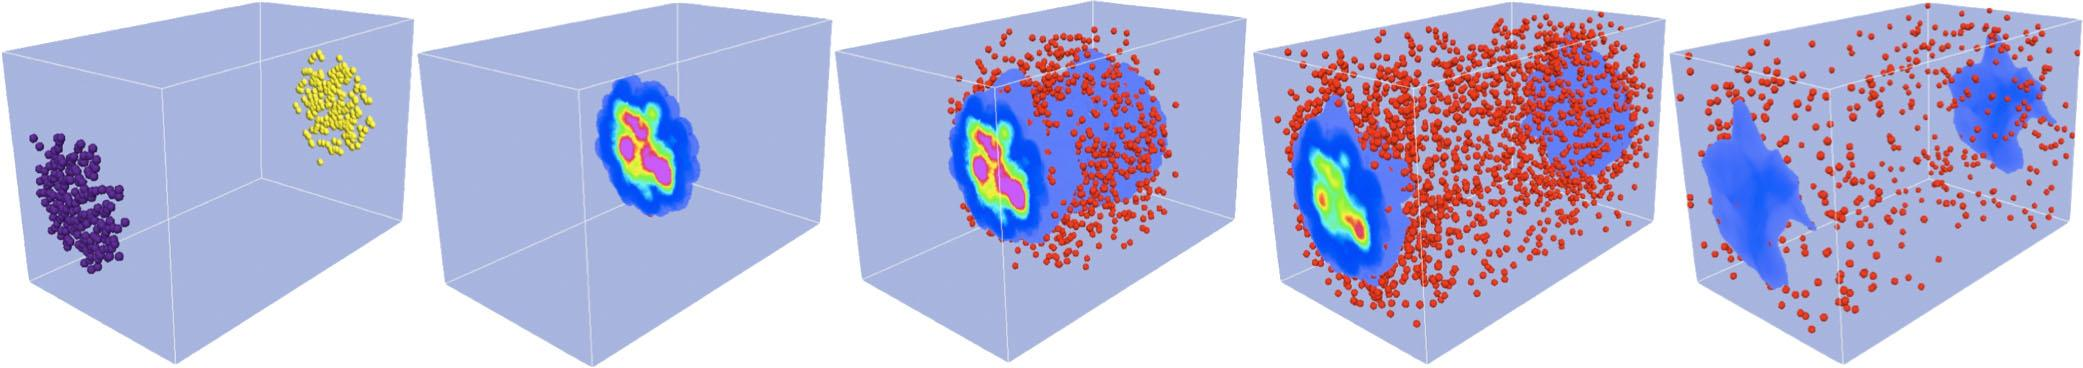
\includegraphics[width=\textwidth]{evolution} \\
  (a) 0 fm/c   \hspace{.1\textwidth}
  (b) 0.5 fm/c \hspace{.1\textwidth}
  (c) 8 fm/c   \hspace{.1\textwidth}
  (d) 16 fm/c  \hspace{.1\textwidth}
  (e) 22 fm/c
  \caption{Simulation of a gold-gold collision at $\sqrt{s}=200$ GeV. Projectile nucleus (purple) collides with target nucleus (yellow) and produces a QGP (heat map). 
  Red spheres indicate cooler hadron resonance gas. Figure from \cite{iss}.}
  \label{fig:evolution}
\end{figure*}

Consider as an example two nuclei with atomic mass numbers $A$ and $B$ which have been accelerated to $\beta=0.9999$ times the speed of light and travel towards
each other along an imaginary beam axis. When viewed from the laboratory frame, the nuclei are Lorentz contracted along the beam-axis by a Gamma-factor 
$\gamma \approx 70$ and thus appear highly compressed \cite{kolb}. 

In the rest frame of each nucleus, the nuclei are described by the multi-body nuclear wavefunctions $\Psi_{A}$ and $\Psi_{B}$ with normalization condition  
\begin{equation}
\int d\vec{x}_1 ... d\vec{x}_A \left | \Psi_A(\vec{x}_1,...,\vec{x}_A) \right|^2 = A.
\end{equation}

The act of collision collapses these wavefunctions and samples a discrete set of nucleon coordinates,
\begin{equation}
 \Psi_{A} \rightarrow \{\vec{x_1},...,\vec{x}_{A}\} ~~~~ \mbox{and} ~~~~ \Psi_{B} \rightarrow \{\vec{x_1},...,\vec{x}_{B}\}
\end{equation}
depicted in panel (a) of FIG. \ref{fig:evolution}. These nucleon configurations may either partially or fully overlap in the moment of collision allowing for various numbers of nucleon 
collisions in a single nucleus-nucleus collision. This first instant of impact defines the collision starting time $\tau=0$ fm/c in units of longitudinal proper time $\tau^2 = t^2-z^2$.

The struck or ``wounded'' nucleons which participate in the collision penetrate each other in the first fraction of a fm/c and liberate quarks and gluons described by 
their nuclear structure functions. These primary quarks and gluons generate secondary partons which are deposited in the plane transverse to the beam axis centered 
at the collision epicenter. The exact physical processes describing these early-time dynamics remain poorly understood and numerous theoretical models exist. We 
discuss two such models for initial particle production in section \ref{sec:initial_condition_models}. 

The initial partonic fireball at incremental time $\tau=0^+$ fm/c is lumpy in the transverse plane and flattened along the beam axis. Transverse fluctuations in the 
density of produced partons reflect fluctuations in configurations of nucleons within the colliding nuclei. 

The secondary energetic partons quickly rescatter and reach thermal equillibrium if the interactions are sufficiently strong. Studies suggest that thermalization 
occurs rapidly in relativistic heavy-ion collisions and sets in around $\tau_{themal} \approx 0.6$ fm/c in $\sqrt{s} = 200$ GeV gold-gold collisions \cite{Heinz:2001xi}.

\subsection{Hydrodynamic evolution}

Once the system reaches thermalization, relativistic hydrodynamics can be used to evolve the thermalized state forward in time (FIG. \ref{fig:evolution} panels b-e). The hydrodynamic equations of motion 
are a set of conservation equations which conserve the flow of four-momentum and net baryon current,
\begin{equation}
 \partial_\mu T^{\mu\nu} = 0 ~~~~~\mbox{and}~~~~~ \partial_\mu j_B^\mu = 0.
\end{equation}

In the ideal (inviscid) limit, the energy momentum tensor and net baryon current can be decomposed as,
\begin{eqnarray}
 \label{energymomentum_tensor}
 \cr T^{\mu\nu} &=& (\varepsilon + p) u^\mu u^\nu - p g^{\mu\nu} \\
 j_B^\mu &=& n u^\mu
\end{eqnarray}
where $\varepsilon$ denotes the system's energy density, $p$ the pressure, $u^\mu$ the fluid four-velocity, $n$ the local baryon density and $g^{\mu\nu}$ the metric 
tensor \cite{kolb}.

Altogether we are left with $5$ equations of motion to describe $6$ field quantities ($\varepsilon$, $p$, $u^1$, $u^2$, $u^3$ and $n$).
The system of equations is closed by adding an additional thermodynamic relation between two of the thermal field quantities, e.g. energy density and pressure. 
This additional relation is known as the equation of state (EOS).

Quite conveniently, the EOS of high temperature, thermal QCD is directly calculable from the QCD Lagrangian using the method of Lattice QCD. The partition function
is expressed in terms of the vaccuum to vaccuum transition amplitude of quark and gluon fields in the Feynman path integral formalism and solved numerically on a
discrete grid. Once the partition function is known, the energy density, entropy density, pressure and temperature are easily interrelated. 

This high temperature EOS is used to model hot and dense regions of the fireball above the critical QGP phase transition temperature $T_c$. At low temperatures,
the QGP EOS is matched to a hadron resonance gas EOS which describes the fluid dynamic behaviour of the QGP once it hadronizes into a dillute gas of bound quark
states. In this manner, the hydrodynamic model naturally describes the complicated dynamics of hadronization which are extremely difficult to model microscopically.

\subsection{Transition to Boltzmann transport}

\begin{figure*}
 \includegraphics[height=0.2\textwidth]{collision1}
 \includegraphics[height=0.2\textwidth]{collision2}
 \includegraphics[height=0.2\textwidth]{collision3}
 \includegraphics[height=0.2\textwidth]{collision4}
 \caption{\label{fig:spacetime} From left to right: (a) nuclei overlap in the transverse plane separated by impact parameter $b$, (b) elliptic overlap
 region drives elliptic flow, (c) discrete nucleons generate distorted, e.g. triangular, fireballs, (d) triangular fireballs drive corresponding triangular flow.}
\end{figure*}

As the system evolves hydrodynamically it expands and cools. The low temperature system eventually becomes that of a hadron resonance gas (FIG. \ref{fig:evolution} panels c-e). While the QGP is a 
roughly homogenous mixture of quarks and gluons, the hadron resonance gas is a complicated, heterogeneous mixture of hadrons and hadronic resonances. Inelastic collisions 
amongst these particles alter the system's chemical composition and drive the system away from chemical equillibirum. 

For these reasons, it is common to switch from hydrodynamics to a Boltzmann description below the QGP phase transition temperature $T_c$ \cite{bass-dumitru}. Boltzmann dynamics naturally 
incorporate chemical nonequillibrium and allow for a more detailed description of the system's low temperature evolution.

To switch from hydrodynamic fields to discrete molecular dynamics, the hydrodynamic medium is first ``particleized''. Particles are sampled from the Cooper-Frye formula 
which describes the particle spectra along a freeze-out hypersurface of constant temperature,
\begin{equation}
 \label{cooper_frye}
 E \frac{dN_i}{d^3p} = \int_\sigma f_i(x,p) p^\mu d^3\sigma_\mu.
\end{equation}
In equation \ref{cooper_frye}, $f_i$ is the particle distribution function, $p^\mu$ is the local fluid four-momentum and $d^3\sigma_\mu$ characterizes an element of the freezeout hypersurface. Equation
\ref{cooper_frye} is integrated over the full freezeout hypersurface to sample particles from the fluid which are then piped into Boltzmann transport simulations.

The Boltzmann equation simulates all elastic and inelastic collisions between the sampled particles until the system becomes too dillute to continue interacting. In symbollic
form it can be written as,
\begin{equation}
 \label{boltzmann_eqn}
 \frac{df_i(x,p)}{dt} = \mathcal{C}_i (x,p),
\end{equation}
where $f_i(x,p)$ is the distribution function of the $i^\mathrm{th}$ particle species and $\mathcal{C}_i$ is the corresponding collision kernel which describes all source 
terms in a collision.

After the particles finish interacting, their positions, momenta and particle ID's are recorded and stored to file. This mock experimental data is then compared with real
data, and free parameters of the model are tuned to optimally replicate reality. The quantities of interest in such a procedure are thus under constrained parameters of 
the model. 

In the next section, I talk about one such quantity, the hydrodynamic specific shear viscosity $\eta/s$ which arises from dissipative corrections to the ideal decomposition of
the energy-momentum tensor in equation \ref{energymomentum_tensor}. A proper description of these viscous corrections is a lengthy discussion in and of itself, and we thus 
sweep these details under the rug for the sake of brevity. Suffice to say, the QGP shear viscosity $\eta/s$ alligns with our classical notions of fluid viscosity.

Model to data extractions of $\eta/s$ indicate that the shear viscosity of the QGP is astonishingly small. Current estimates of the QGP shear viscosity place bounds 
$0.08 \le \eta/s \le 0.20$. For comparison, the value of $\eta/s$ for water at the liquid-gas phase transition is $\eta/s \approx 2$ \cite{bhalerao:2014owa}. The QGP has consequently been called the 
``perfect fluid''. We discuss current methods for extracting $\eta/s$ from model to data comparisons and isolate the largest source of uncertainty in these extractions.

\section{Constraining the QGP viscosity}

When a nuclear collision is viewed along the beam axis, the nuclei collide and overlap in the plane orthogonal to the beam axis, offset by a random separation vector $b$ 
(FIG. \ref{fig:spacetime} panel a). The resulting almond shaped fireball is highly anisotropic and is described by energy density gradients which are larger along its short axis. These 
gradients drive more flow along the fireball's short axis than its long axis and thus generate elliptic flow (FIG. \ref{fig:spacetime} panel b).

Additional fluctuations in the distribution of nucleons within each nucleus distort the almond shape of the produced fireball. These fluctuations are uncorrelated with the 
impact parameter geometry of the collision and hence cannot be characterized by a single elliptic shape. For example, it's entirely possible that random nucleon fluctuations
generate a triangular fireball with corresponding triangular flow profile (FIG. \ref{fig:spacetime} panels c and d). 

It's worth stressing that this conversion from spatial anisotropy to flow anisotropy is a characteristic signature of hydrodynamic behaviour. The efficiency of conversion
tells us about the strength of dissipative forces in the fluid, most notably the fluid shear viscosity $\eta/s$.

\subsection{Viscosity from anisotropic flow}

Hydrodynamic conversion from spatial anisotropy to momentum anisotropy becomes easier to quantify if we first decompose the initial and final states using an azimuthal 
Fourier expansion. 

The initial state spatial anisotropy is characterized by the Fourier eccentricity harmonics $\varepsilon_n$ given by,
\begin{equation}
 \varepsilon_n e^{-i n \Phi_n} = -\frac{\int dx\,dy\,r^n e^{i n \phi} s(x,y)}{\int dx\,dy\, r^n s(x,y)}
\end{equation}
where $n$ denotes the eccentrcity harmonic mode number, $\Phi_n$ denotes the direction of the steepest density gradient and $s(x,y)$ the event's transverse entropy density
(often energy is used as well). Examples of eccentricity harmonics two, three, four and five are shown in FIG. \ref{fig:harmonics}.

An analogous expansion for the final state flow anisotropy yields the flow coefficients $v_n$,
\begin{equation}
 v_n(y) e^{i n \Psi_n(y)} = \frac{\int p_T dp_T d\phi_p e^{i n \phi_p} \frac{dN}{dy p_T dp_T d\phi_p}}{\int p_T dp_T d\phi_p \frac{dN}{dy p_T dp_T d\phi_p}}
\end{equation}
where $n$ denotes the anisotropic flow mode number, $\Psi_n$ denotes the angle of maximum flow, $p_T$ a particle's transverse momentum and 
$y=\tfrac{1}{2}\log(\tfrac{E+p_z}{E-p_z})$ its rapidity.

Hydrodynamic expansion converts n-th order eccentricity $\varepsilon_n$ into n-th order harmonic flow $v_n$ with a conversion efficiency that's proportional to the fluid's
specific shear viscosity $\eta/s$,
\begin{equation}
 \label{linear_response}
 v_n/\varepsilon_n \propto \eta/s.
\end{equation}

Thus \emph{if} one possessed a realistic initial condition model from which they could calculate the eccentricity harmonics $\varepsilon_n$, \emph{and} they had faith 
in their hydrodynamic description of the produced plasma, \emph{then} they could calculate the flow harmonics $v_n$ from equation \ref{linear_response} for different values 
of the QGP viscosity and find the one which optimally fits experimental flow measurements.

Somewhat surprisingly, the biggest obstacle in this whole procedure is not the derivation of relativistic viscous hydrodynamics, or calculations of the lattice equation
of state or even microscopic descriptions of the hadron resonance gas - it's a description of the system's hydrodynamic initial conditions. 

\begin{figure}[t]
 \includegraphics[width=0.15\columnwidth]{e2-crop} \hspace{.01\columnwidth} 
 \includegraphics[width=0.23\columnwidth]{e3-crop} \hspace{.01\columnwidth}
 \includegraphics[width=0.21\columnwidth]{e4-crop} \hspace{.01\columnwidth}
 \includegraphics[width=0.24\columnwidth]{e5-crop}\\
 \flushleft
 \vspace{-0.1in}
 \hspace{0.08\columnwidth} 2 \hspace{0.19\columnwidth} 3 \hspace{0.21\columnwidth} 4 \hspace{0.22\columnwidth} 5
 \caption{\label{fig:harmonics} Diagrams of the second, third, fourth and fifth azimuthal Fourier harmonics. The angular resolution increases with increasing harmonic number.}
\end{figure}

\section{Initial condition models}
\label{sec:initial_condition_models}

Hydrodynamic initial conditions describe the thermal state of the QGP fluid at the QGP thermalization time $\tau_{therm} \approx 1$ fm/c. These initial condition models
fall into two general categories - dynamical models which calculate the initial state of the system at time $\tau=0$ fm/c and explicitly simulate the pre-equillibrium 
dynamics which drive the system to thermalization, and effective models which omit early-time dynamics to generate profiles of energy or entropy \emph{at} the QGP thermalization time. 
Historically, effective models have been preferred for their simplicity, and despite recent advances in pre-equillibirum transport theory, remain the most popular.

\subsection{Glauber modeling}

The most famous effective model for hydrodynamic initial conditions is the well known Glauber model (for an overview see \cite{glauber}). The Glauber model asserts that particle production in nucleus-nucleus 
collisions scales with a linear combination of ``hard'' and ``soft'' collision processes. 

For hard processes, it's natural to assume that the number of produced particles scales with the number of binary nucleon-nucleon collisions. Hard processes correspond
to large momentum transfer and are well localized in the collision. This means that interference effects can be safely ignored. In contrast, soft processes are strongly 
affected by coherence effects and should not scale linearly with the number of binary collisions.

Soft processes are particularly challenging because they are inherently non-perturbative (strong coupling) and thus cannot be calculated using the usual tools
of perturbative QCD. The Glauber model thus adopts an ansatz for soft particle production and scales soft processes with the number of wounded nucleons, i.e. nucleons 
which participate in at least one collision. In this picture, successive nucleon collisions change the excited state of the wounded nucleon but do not contribute to 
overall particle production. The excited nucleons become de-excited once they leave the interaction region and thus generate secondary densities proportional to the 
initial density of wounded nucleons.

Binary collisions and wounded nucleons are typically counted by considering all possible pairs of nucleon-nucleon collisions which occur with probability
\begin{equation}
P_{coll}=
\begin{cases}
  1 &\mbox{if } b \le \sqrt{\sigma^{inel}_{NN}/\pi} \\ 
  0 &\mbox{if } b > \sqrt{\sigma^{inel}_{NN}/\pi},
\end{cases}
\end{equation}
where $b$ denotes the nucleon-nucleon impact parameter and $\sigma^{inel}_{NN}$ the inelastic nucleon-nucleon cross section.

These particle interactions are then converted to smooth density profiles by depositing a small Gaussian about each wounded nucleon coordinate and binary
collision vertex. The resulting density profiles are then projected onto the transverse plane yielding,
\begin{eqnarray}
 \label{BC_WN}
 \cr BC(x,y) &=& \sum_{i=1}^{N_{coll}} \frac{1}{\sqrt{2 \pi \sigma^2}} e^{ -|\vec{r}_\perp-\vec{r}_{i\perp}|^2/2 \sigma^2 }   \\
 WN(x,y) &=& \sum_{i=1}^{N_{part}} \frac{1}{\sqrt{2 \pi \sigma^2}} e^{ -|\vec{r}_\perp-\vec{r}_{i\perp}|^2/2 \sigma^2 } .
\end{eqnarray}
where the Gaussian deposition width $\sigma$ is a free parameter.

The entropy (or often energy) density of the fireball is finally set proportional to a linear combination of the binary collision and wounded nucleon densities,
\begin{equation}
 \frac{dS(x,y)}{d^2r_\perp dy} \propto \frac{1-\alpha}{2} WN(x,y) + \alpha\, BC(x,y),
\end{equation}
where $dS(x,y)/d^2r_\perp dy$ is the fireball's transverse entropy density, $\alpha$ is a unitless tunable parameter and $\vec{r}_\perp$ is a position in the 
transverse plane. We note that the Glauber model projects all densities onto the transverse plane and thus does not resolve any structure along the collision beam axis.

\subsection{Color-Glass Condensate theory}

In Color-Glass Condensate theory, the transverse entropy density at mid-rapidity scales with the density of secondary gluons produced by individual gluon-gluon interactions.
This density depends on the number of available states, and in turn on the local gluon distribution functions in each colliding nucleon pair. These gluon distribution 
functions are connected to the underlying nuclear geometry through a parameter known as the saturation scale $Q_s$ via it's dependence on the nuclear thickness 
functions $T_{A}$ and $T_{B}$ which describe the transverse opacity of participant nucleons in each nucleus,
\begin{equation}
 \label{thickness}
 T_A(x,y) = \sum\limits_{i=1}^{A} \frac{1}{\sqrt{2 \pi \sigma^2_p}} e^{ -|\vec{r}_\perp-\vec{r}_{i\perp}|^2/2 \sigma_{p}^2 }.  
\end{equation}

There exist a number of Color-Glass Condensate realizations which convert the nuclear thickness functions $T_{A}$ and $T_{B}$ defined by equation \ref{thickness} into 
secondary gluon densities and hence entropy densities at mid-rapidity, but we only discuss one for the sake of brevity.

The Kharzeev-Levin-Nardi (KLN) model is one well known implementation of Color-Glass Condensate effective field theory \cite{KLN}. In the KLN model, the gluon saturation scale 
$Q_s$ is parameterized by
\begin{equation}
 Q^2_s(x;{\bf r}_\perp) = 2\, \mbox{GeV}^2 \left( \frac{T({\bf r}_\perp)}{T_0} \right) \bigg( \frac{x_0}{x} \bigg)^\lambda,
\end{equation}
where $T_0=1.53$ fm$^{-2}$ and $x_0 = 0.01$. Here $x=p_\perp \exp(\pm y)/\sqrt{s}$ is the light-cone momentum fraction of a gluon and $\lambda$ is a 
dimensionless parameter tuned to fit the observed hadron multiplicity in central collisions.
 
The gluon distribution functions are then expressed in terms of the gluon saturation scale as,
\begin{equation}
 \phi(x,k^2_\perp,{\bf r}_\perp) \sim \frac{1}{\alpha_s(Q_s^2)}\frac{Q_s^2}{\max(Q_s^2,k_\perp^2)}
\end{equation}
where $k_\perp$ is the transverse momentum of a gluon and $\alpha_s$ specifies the strength of the coupling constant. 

Once the gluon distribution functions are known, the density of produced gluons is calculated by integrating a gluon fusion term over the full collision phase space,
\begin{eqnarray}
 \cr \frac{dN_g}{d^2r_\perp dy} &=& \frac{2 \pi^2}{C_F} \int^{p_\perp^{max}} \frac{d^2 p_\perp}{p_\perp^2} \int^{p_\perp} \frac{d^2 k_\perp}{4} \alpha_s(Q_s^2) \\
 &\times& \phi_1(x_1,({\bf p}_\perp + {\bf k}_\perp)^2/4; {\bf r}_\perp) \\
 &\times& \phi_2(x_2,({\bf p}_\perp - {\bf k}_\perp)^2/4; {\bf r}_\perp),
\end{eqnarray}
where $C_F$ is a color factor, $\phi_1$ and $\phi_2$ are the gluon distribution functions of each nucleus and $p_\perp = p_\perp^1 + p_\perp^2$ and 
$k_\perp = p_\perp^1 - p_\perp^2$ denote the primary transverse gluon momentum in center of mass coordinates. This furnishes the transverse entropy density up to an 
overall normalization factor,
\begin{equation}
 \frac{dS(x,y)}{d^2r_\perp dy} \propto \frac{dN_g}{d^2r_\perp dy}.
\end{equation}

\section{The case for new I.C. models}

Originally, collective flow behaviour was thought to only exists in collisions of \emph{heavy} nuclei where the produced fireball is sufficiently large and dense to reach 
a state of local thermal equillibrium. Proton-lead collisions, on the other hand, were thought to be too small to produce any signatures of collective flow.

It thus came as a great surprise when proton-lead collisions - which were scheduled primarily as a calibration run for larger collisions - produced significant signs of 
collective behaviour. This discovery raised several key questions within the heavy-ion community:
\begin{itemize}
 \item Do small collision systems produce a QGP? 
 \item Are the hydrodynamic equations of motion valid in small systems?
 \item If so, how do we unite large and small systems under a single theoretical framework?
\end{itemize}

The application of the Glauber and KLN models to the full range of collision systems measured at RHIC and the LHC has been carried out with mixed success. The KLN model
struggles to replicate the full spectrum of measured anisotropic flow coefficients and the Glauber model has problems describing collisions of deformed nuclei, while 
both models do a poor job describing small collision systems. There is in fact only one model, a CGC relative called IP-Glasma, which has provided an excellent 
description of flow harmonics in heavy nuclei at RHIC and the LHC, but even its application to smaller collision systems remains uncertain.

Perhaps even more worrisome than flow inconsistencies, which may simply result from applying hydrodynamics where it's not applicable, are inconsistencies in the description 
of particle production; there are models which provide satisfactory descriptions of particle production in proton-proton collisions, and there models which provide 
satisfactory descriptions of particle production in heavy-ion collisions, but very few models do both simultaneously. 

Yet if we look at the density of nuclear overlap in heavy-ion collisions, we see that there are regions of overlap which are identical to those found in light-nucleus 
collisions. For example, isolated proton-proton collisions frequently occur around the edges of gold-gold collisions. In fact, a wide range of ``$n$-on-$m$'' nucleon-nucleon 
collisions occur \emph{inside} a single heavy-ion collision. It's thus hard to trust any model which claims to simulate the overall distribution of matter in large nucleus-nucleus collisions without simulatenously describing the 
distribution of matter produced by all collision sub-fragments. 

\section{Particle production as a mapping}

\begin{figure}
 \includegraphics[height=0.19\textwidth]{motivation1-crop}\\
 \caption{\label{fig:motivation_beam} Beam view: imaginary Cartesian grid superimposed on top of nuclear overlap region}
 \includegraphics[height=0.13\textwidth]{motivation2-crop}
 \caption{\label{fig:motivation_side} Side view: Example of a grid cell containing a localized three-on-two nucleon collision}
\end{figure}

We now firm up the motivation for a composite description of the QGP fireball with a heuristic argument. Imagine that we have the freedom to construct and collide any 
$m$-on-$n$ combination of $m$ projectile and $n$ target nucleons. The experiment is performed and the average number of charged particles in a fixed interval about 
mid-rapidity $|\eta|< \eta_{max}$ recorded as $N_{ch}(n,\, m)$.

For example, the simplest combination of projectile and target nucleons is a $1$-on-$1$ collision of two protons $N_{ch}(1,\, 1)$. A single proton is then added to the 
target nucleus, positioned just behind the original target proton in line with the beam axis, and the collision is repeated at the 
same beam energy yielding a new measurement for a $1$-on-$2$ collision $N_{ch}(1,\, 2)$.

At this point you can probably see where we are headed. We continue to extend the projectile and target nuclei by adding  protons to the column of existing protons 
and record the number of charged particles measured in the collision. We thus build up a two dimensional surface that describes particle production for any $m$-on-$n$ 
collision. We will now argue that this surface is all we need to approximate entropy deposition in the early stages of a generic nucleus-nucleus collision. 

\section{Reverse engineering the fireball}
\label{sec:reverse_engineering}

Hydrodynamic simulations indicate that, to good approximation, the simulation's initial entropy is a close proxy for final state particle production \cite{Song:2008si}. 
This linear correspondence is of course affected by small corrections from viscous entropy production and inelastic hadron resonance gas collisions, but nevertheless 
holds quite well. 

We use this linear relation to revert equation \ref{charged_particles} into a statement about initial entropy deposition,
\begin{equation}
 \label{entropy_mapping}
 N_{ch}(n,\, m) \propto S(n,\, m),
\end{equation}
where $S$ is the initial entropy deposited in the rapidity interval where $N_{ch}$ is measured.

We now imagine a realistic collision of two heavy nuclei which overlap at some non-zero impact parameter in the transverse plane. We can superimpose an imaginary
Cartesian grid on top of this overlap region and model each grid cell as an $m$-on-$n$ collision of projectile and target nucleons 
(see FIG. \ref{fig:motivation_beam}, \ref{fig:motivation_side}). We can then simply read off the value of entropy deposition from equation \ref{entropy_mapping} 
for each grid cell and renormalize the entire profile to account for the unknown entropy to particle number conversion factor.

Unfortunately, nature will not allow us to construct elongated stacks of protons or even control the orrientation of nuclei when they collide. Therefore we cannot simply
measure particle production for every possible $m$-on-$n$ collision. Instead, we start from a suitably flexible ansatz for entropy deposition and constrain our ansatz 
using the full gamut of nucleus-nucleus multiplicity data.

\subsection{Ansatz for entropy deposition}

In our original line of reasoning, we formulated the problem in terms of global quantities such as the \emph{number} of nucleons in the projectile and target.
We can easily recast expression \ref{entropy_mapping} locally by replacing nucleon number with nuclear density
\begin{equation}
 \label{mapping}
 \frac{dN_{ch}}{d\eta} \propto \frac{dS}{d\eta} \bigg|_{\tau=\tau_0} \propto f(T_A,T_B),
\end{equation}
where $T_A$ and $T_B$ are the thickness functions
\begin{equation}
 T_{A,B}(x,y) = \int dz\, \rho_{A,B}(x,y,z).
\end{equation}
At first glance we might worry that the function $f$ in equation \ref{mapping} could be \emph{any} mapping $f:\mathbb{R}^2 \rightarrow \mathbb{R}$. However, it's easy to see that the mapping
must obey a number of constraints,
\begin{enumerate}
 \item The collision would still be the same if we rotated our lab frame $180^{\circ}$ and thus our mapping should be symmetric under interchange of $T_A$ and $T_B$.
 \item Denser collisions should deposit more matter and thus the mapping should increase monotonically with respect to $T_A$ and $T_B$.
 \item The mapping should respect sensible limits; if either $T_A$ or $T_B$ goes to zero, $f(T_A,T_B)$ should also go to zero.
\end{enumerate}

We now consider an imaginary collision between a single nucleon and a stack of \emph{many} nucleons, e.g. a proton hitting a neutron star. Clearly, we expect particle
production in such a collision to scale with the integrated density of the proton and not the integrated density of the neutron star. 

The example, while extreme, illustrates an important point. Charged particle production should \emph{attenuate} in highly asymmetric collisions. With the aforementioned
constraints and scaling considerations in mind, we consider for $f$ the functional form
\begin{equation}
 f \equiv M_p(T_A,T_B) = \left(\frac{T_A^p + T_B^p}{2} \right) ^{1/p}
\end{equation}
known as the generalized mean. The dimensionless parameter $p$ smoothly interpolates the space of vector two-norms, e.g.
\begin{equation}
  M(p; T_A, T_B) =
  \begin{cases}
    \dfrac{2\, T_A T_B}{T_A + T_B} & p = -1 \text{ (harmonic mean)}, \\[2ex]
    \sqrt{T_A T_B} & p = 0 \text{ (geometric mean)}, \\[2ex]
    \dfrac{T_A + T_B}{2} & p = 1 \text{ (arithmetic mean)}, \\[2ex]
  \end{cases}
\end{equation}
and assumes the limiting values,
\begin{eqnarray}
 \lim\limits_{p\rightarrow -\infty}M(p;T_A,T_B) \rightarrow \min{(T_A,T_B)} \\
 \lim\limits_{p\rightarrow \infty}M(p;T_A,T_B) \rightarrow \max{(T_A,T_B)}.
\end{eqnarray}
More generally, the parameter $p$ quantifies the attentuation of particle production in locally asymmetric $(T_A \ne T_B)$ regions of a collision. 

We stress that this proposed ansatz exhibits markedly different scaling behaviour from the well known Glauber model. While the Glauber model deviates from participant
nucleon scaling by modifying symmetric regions of the mapping where $T_A \approx T_B$, the generalized mean ansatz does exactly the opposite and parameterizes 
modifications to asymmetric regions of the mapping where $T_A \ll T_B$ and $T_B \ll T_A$. We now detail the construction of a new I.C. model built on the generalized mean ansatz.

\begin{figure}
 \includegraphics[width=\columnwidth]{saturation}
\caption{\label{fig:saturation} Attentuation of the reduced thickness. Thickness $T_B$ is fixed to one (in arbitrary units) while $T_A$ is varied. The corresponding $T_R$ are shown for 
 $p=1,0,-1$ (green, blue, and red).}
\end{figure}

\section{Trento, a new model for I.C.}

\begin{figure*}[t]
  \includegraphics{multdist}
  \caption{
    \label{fig:multdist}
    Multiplicity distributions for proton-proton, proton-lead, and lead-lead collisions.  The blue histograms
    are \protect\trento\ results from $10^6$ minimum-bias events for each collision system, all with reduced
    thickness parameter $p = 0$ (geometric mean) and gamma fluctuation parameter $k = 1.25$.  The normalization
    constants indicated in the legends are tuned to match the experimental distributions
    (points with error bars) from ALICE \cite{Aamodt:2010ft,Abelev:2014mda}.
  }
\end{figure*}

Motivated by the previous discussion we introduce the \emph{reduced thickness},
\begin{equation}
 T_R(p;T_A,T_B) \equiv \left(\frac{T_A^p + T_B^p}{2} \right) ^{1/p},
\end{equation}
so named because it uses the generalized mean to reduce two thicknesses $T_A$, $T_B$ to a third profile with units of thickness. This function also furnishes the name of our
model \trento, for thickness-reduced event-by-event nuclear topology. 

The nuclear thickness functions $T_A$ and $T_B$ are calculated by sampling realistic nucleon configurations shifted by collision impact parameter $b$ for each 
nucleus using uncorrelated Woods-Saxon sampling or correlated nucleon configurations when available.

Each nucleon is then described by a density profile,
\begin{equation}
 \rho_{A,B} = \rho_{proton}(x \pm b/2,y,z)
\end{equation}
where the integral $\int dz \rho_{proton}$ either has a closed form or may be evaluated numerically, so that the proton thickness functions can calculated.
The nucleons are then determined to collide with probability,
\begin{equation}
 P_{coll} = 1 - \exp \left[ -\sigma_{gg} \int dx dy \int dz \rho_A \int dz \rho_B \right]
\end{equation}
where the integrand denotes the proton-proton overlap density and $\sigma_{gg}$ an ``effective'' glue-glue cross section tuned to replicate the experimentally 
measured nucleon-nucleon cross section $\sigma_{NN}$.

$P_{coll}$ is sampled once for each \emph{pair} of projectile and target nucleons, and nucleons which \emph{do not} participate in at least once pairwise collision are 
discarded. The remaining nucleons are assigned a \emph{fluctuated} thickness function,
\begin{equation}
 T_{A}(x,y) = \sum\limits_i \gamma_i \int dz\, \rho_{A}(x-x_i,y-y_i,z-z_i),
\end{equation}
where $\gamma_i$ is an independent random number sampled from a Gamma distribution with unit mean,
\begin{equation}
 P(\gamma;k) \propto \gamma^{k-1} e^{-\gamma/k}
\end{equation}
with shape parameter $k>0$ to be fixed by experiment. These Gamma fluctuations, commonly employed by Glauber simulations, replicate large negative binomial fluctuations 
observed in minimum bias proton-proton collisions (note that the Gamma distribution is the continuous analogue of the negative binomial distribution).

The QGP entropy density at the  thermalization time is finally calculated from equation \ref{mapping},
\begin{equation}
 \frac{dS}{d\eta} \bigg|_{\tau=\tau_0} \propto T_R(p;T_A,T_B).
\end{equation}

This completes the specification of the model. It's worth noting that the arguments outlined above are not specific to certain types of nuclei and thus should hold 
for \emph{any} $A$ on $B$ collision. We require only that (i) the collision occur at sufficiently high energies where the eikonal approximation is valid and (ii) 
thermalization is sufficiently rapid to preserve locality. We now apply the model to recent nucleus-nucleus collisions at the LHC where these conditions are expected to hold.

\section{Results}

We now demonstrate \trento's ability to simultaneously describe a wide range of collision systems. Note that the reduced thickness parameter $p$, gamma fluctuation 
parameter $k$, and nucleon profile $\rho_\text{proton}$ are not rigorously constrained---to do so would require a systematic model-to-data comparison which is beyond the 
scope of this work. Therefore, the following results do not necessarily represent the best-fit of the model to data.

\begin{figure*}[t]
  \includegraphics{eccentricity}
  \caption{
    \label{fig:eccen}
    Left and middle plots:  Eccentricity harmonics $\varepsilon_2$, $\varepsilon_3$ as function of centrality
    for reduced thickness parameters $p = 1$, 0, $-1$ (green, blue, and red).  Right plot:  Ratio of rms eccentricities
    $\eccratio$ against the experimentally allowed region (grey band) from \cite{Retinskaya:2014zea}.  Note centrality
    axis has different range in the ratio plot.
  }
\end{figure*}

In section \ref{sec:reverse_engineering} we explained that the experimentally observed charged-particle multiplicity $\nch$ is to a very good approximation proportional to 
the total initial entropy \cite{Song:2008si}, and hence should scale with the integrated reduced thickness:
\begin{equation}
  \nch \propto \int dx \, dy \, T_R.
\end{equation}
To compare with experiment, we generate a large ensemble of minimum-bias events, integrate their $T_R$ profiles, and rescale by an overall normalization constant.

The left panel of FIG.~\ref{fig:multdist} shows the $\nch$ distribution from $10^6$ proton-proton simulations
using reduced thickness parameter $p = 0$ (geometric mean), gamma fluctuation parameter $k = 1.25$, and
Gaussian beam-integrated proton density
\begin{equation}
  \int dz \, \rho_\text{proton} = \frac{1}{2\pi B} \exp\biggr( -\frac{x^2 + y^2}{2B} \biggr)
\end{equation}
with effective area $B = (0.6\;\text{fm})^2$.
Proton-lead and lead-lead distributions (middle and right panels) use identical model parameters, except for the overall normalization factor, whose $\sim$20\% variation across collision systems is consistent with differences in experimental beam energy and kinematic cuts (annotated in the figure).

The $\nch$ distributions compare favorably with the corresponding experimental measurements by ALICE \cite{Aamodt:2010ft,Abelev:2014mda} and \trento\ is able to 
simultaneously reproduce the shapes of all three distributions with a single set of parameters. 

Eccentricity harmonics $\varepsilon_n$ are calculated using the definition
\begin{equation}
  \varepsilon_n e^{i n\phi} = -\frac{\int dx \, dy\, r^n e^{i n \phi} \, T_R}{\int dx \, dy \, r^n \, T_R}.
\end{equation}
Figure~\ref{fig:eccen} shows ellipticity $\varepsilon_2$ and triangularity $\varepsilon_3$ for lead-lead collisions as a function of centrality for reduced thickness $p = 1$,~0,~$-1$.  There is a clear trend of increasing eccentricity
(particularly $\varepsilon_2$) with decreasing $p$.  This may be understood by the attenuation property of the
reduced thickness:  as $p$ decreases, asymmetric regions of the collision produce less entropy, which
accentuates the elliptical overlap shape in non-central collisions and enhances their eccentricity.

In addition, we perform the test proposed by \cite{Retinskaya:2014zea}, which uses flow data and hydrodynamic calculations to determine an experimentally allowed band for the ratio of root-mean-square eccentricities $\eccratio$ as a function of centrality.
Among available initial condition models only IP-Glasma consistently falls within the allowed region.
As shown in the right panel of FIG.~\ref{fig:eccen}, \trento\ yields excellent agreement with the allowed band for $p = 0$ (geometric mean).

\section{Summary and Outlook}

In this preliminary exam report we discuss some of the overall goals of high energy nuclear physics, in particular, the effort to extract bulk properties of hot and dense 
nuclear matter from ultra-relativistic nucleus-nucleus collisions. 

Properties are extracted using the techniques of model-to-data comparison in which accurate, albeit underconstrained, models are tuned to optimally replicate experimental 
measurements. The best fit values of the underconstrained parameters are then interpretted as the true values \emph{up errors and uncertainties of the underlying model}.
It is thus critically important that the model provide a faithful description of reality. If any component of the model deviates from reality, the extracted parameters will
inherit the non-physical bias.

We focus on model-to-data extractions of the QGP shear viscosity to entropy ratio $\eta/s$ which suggest that the QGP may be the most ideal (least viscous) fluid in existence.
These models naturally inherrit error from the imperfect theories used to describe each stage of the collision, and hence uncertainties in the assumed model propagate into uncertainties
in the extracted value of $\eta/s$.

The overwhelming source of uncertainty in modern simulations is contributed by poorly constrained models of the QGP initial conditions. Initial conditions are typically constructed from 
``bottom-up'' approaches which use existing theories, e.g. perturbative QCD, to calculate the distribution of matter at the QGP thermalization time. In this report, we 
assume a ``top-down'' approach and parameterize the space of reasonable initial condition models using a well motivated functional form known as the generalized mean. 
While our approach cannot explain how the QGP fireball was formed, it will allow us to constrain the QGP viscosity without adopting one of the many theoretical models in 
circulation.

First results indicate that we are able to simulatenously describe the charged particle multiplicity distributions of proton-proton, proton-lead and lead-lead collisions 
with a level of precision that is unmatched by current theoretical models. Preliminary results also indicate that we will be able to describe the second and third-order
anisotropic flow coefficient $v_2$ and $v_3$, although stronger claims necessitate a rigorous model-to-data comparison which is currently under way. We plan to use this work
to publish tighter constraints on the QGP shear viscosity $\eta/s$ in the coming months.




\bibliography{prelim,duke-qcd-refs/Duke_QCD_refs}


\end{document}
